%-----------------------------------------------------------------------------%
\chapter{\babEmpat}
%-----------------------------------------------------------------------------%

Bab ini berisi tentang hasil penelitian berupa percobaan yang dilakukan dan hasil dari percobaan.

\section{Data}
Data yang digunakan adalah data lokasi access point dari \textit{hotspot} yang ada di fakultas-fakultas di kampus UI. Data tersebut didapat dari DSTI UI. Data yang tersedia berupa informasi lokasi access point, tipe router, dan nama controller-nya.

Contoh: CS-A-1-Lab 1105 | Aruba AP 225 | wagyu.ui.ac.id

Informasi tersebut menggambarkan lokasi access point di Fakultas Ilmu Komputer, gedung A, lantai 1, ruang Lab 1105. Tipe router-nya adalah Aruba AP 225, dan controller-nya ada di wagyu.ui.ac.id.

Data dari DSTI hanya berisi data lokasi \textit{access point} untuk fakultas-fakultas yang ada di {\ui}, tanpa data lokasi hotspot untuk daerah di luar fakultas seperti Balairung atau Rektorat.

\subsection{Data \textit{Access Point}}
Terdapat enam \textit{access point} berbeda yang digunakan di kampus {\ui} yaitu Aruba AP 135, Aruba AP 215, Aruba AP 225, Aruba AP 275, Cisco Aironet 1040 LWAPP, dan Cisco Aironet 1600i LWAPP. Berdasarkan http://www.arubanetworks.com/products/networking/access-points/ untuk Aruba AP 135 mencapai 300 Mbps, Aruba AP 215 dan Aruba AP 225 mencapai 867 Mbps, sedangkan Aruba AP 275 mencapai 1.3 Gbps. Untuk Cisco, berdasarkan https://www.cisco.com/c/en/us/products/collateral/wireless/aironet-1140-series/data_sheet_c78-609338.html dan https://www.cisco.com/c/en/us/products/collateral/wireless/aironet-1600-series/data_sheet_c78-715702.html mencapai 300 Mbps.

\subsection{Olah Data}
Dari data yang didapat tentang lokasi access point kemudian di petakan ke peta untuk mendapatkan koordinat longitude dan latitude-nya. Misalkan untuk Fakultas Ilmu Komputer, gedung A lantai satu, ruang 1105 titik koordinatnya berada pada -6.364724, 106.828851.

\section{Penggambaran Peta Universitas Indonesia}
Peta {\ui} diambil dari Google Maps dengan perbandingan 1:100000.
% (https://www.google.co.id/maps/place/University+of+Indonesia/@-6.3655306,106.8255746,16.65z/data=!4m5!3m4!1s0x2e69ec1a804e8b85:0xd7bf80e1977cea07!8m2!3d-6.3627638!4d106.8270482?hl=en) 

\begin{figure}
	\centering
	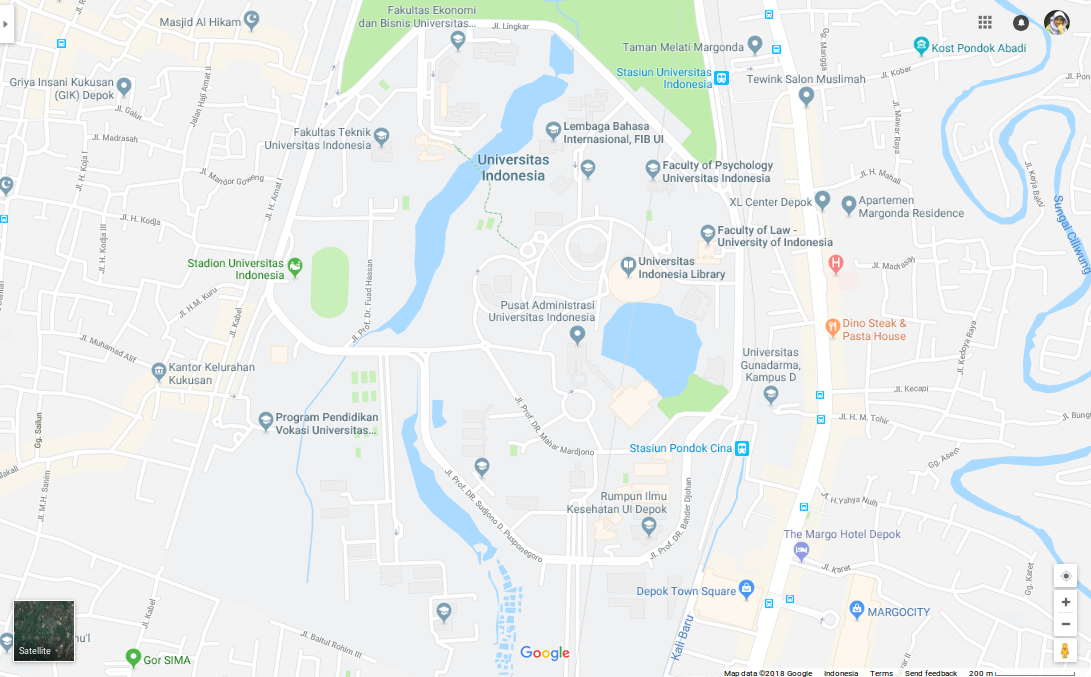
\includegraphics[width=12cm]{pics/ui.png}
	\caption{Peta Kampus Universitas Indonesia Depok}
	\label{fig:ui}
	\cite{ui.map}
\end{figure} 

Gambar di atas merupakan peta kampus {\ui}, Depok. Peta tersebut diambil dari Google Maps pada tanggal 21 Januari 2018 pukul 23:22. Peta tersebut berskala 1:100000.

Tidak semua wilayah dari kampus {\ui}, Depok dimasukkan dalam penelitian ini. Hanya wilayah sekitar fakultas dan stasiun tanpa memasukkan area asrama {\ui} dan area hutan {\ui}.

\section{Menggambarkan Demand dari \textit{Hotspot} Pada Peta}

Warna merah pada peta menggambarkan demand atau daerah yang harus dijangkau oleh \textit{hotspot} UI. Daerah yang digambarkan oleh warna merah tersebut adalah daerah-daerah dalam lingkungan fakultas, area publik, daerah-daerah penghubung antar fakultas, dan area pejalan kaki.

Area yang dipilih menjadi \textit{demand area} adalah daerah yang ramai dengan manusia seperti di stasiun, di halte bis kuning, di dalam bis kuning, perpustakaan, dan lain-lain.

\begin{figure}
	\centering
	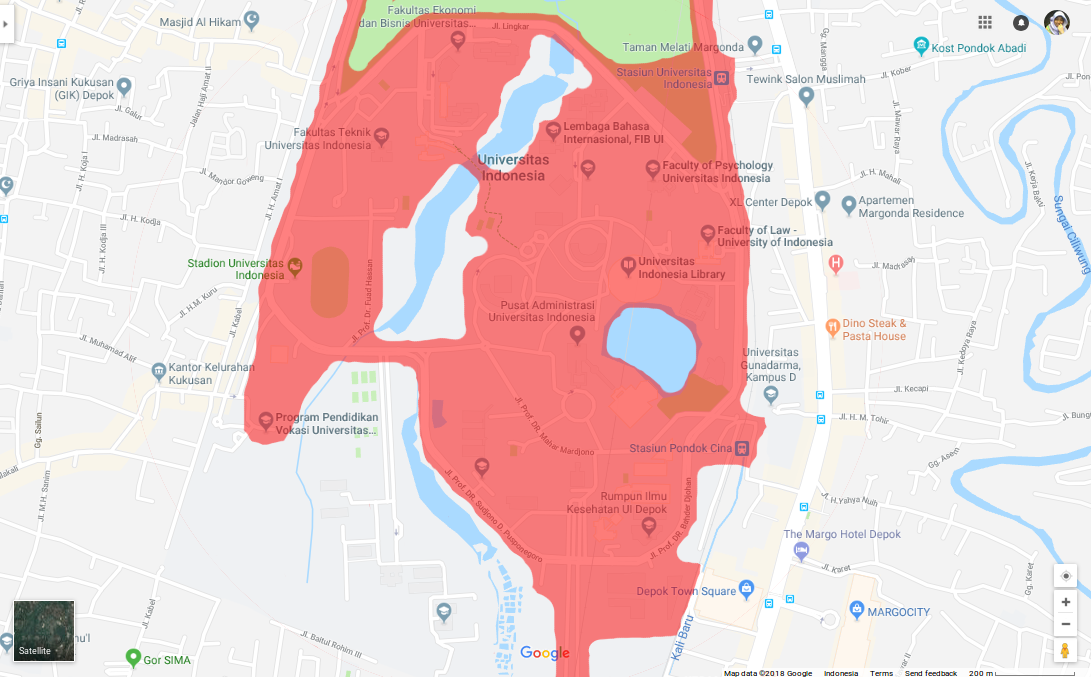
\includegraphics[width=14cm]{pics/ui-demand.png}
	\caption{Peta Kampus Universitas Indonesia dengan \textit{Demand} dari \textit{Hotspot}}
	\label{fig:uiDemand}
\end{figure} 

\section{Menambahkan Lokasi \textit{Hotspot} dan Bobot untuk Weighted Voronoi Diagram}

Berdasarkan data dari DSTI tentang lokasi \textit{access point} yang ada di kampus {\ui}, digambarkan setiap lokasi tersebut dalam peta kampus {\ui} Depok. Lokasi dari \textit{access point} digambarkan dengan titik berwarna hitam. Lokasi \textit{access point} yang digambarkan hanya \textit{access point} yang ada di lantai satu.

\begin{figure}
	\centering
	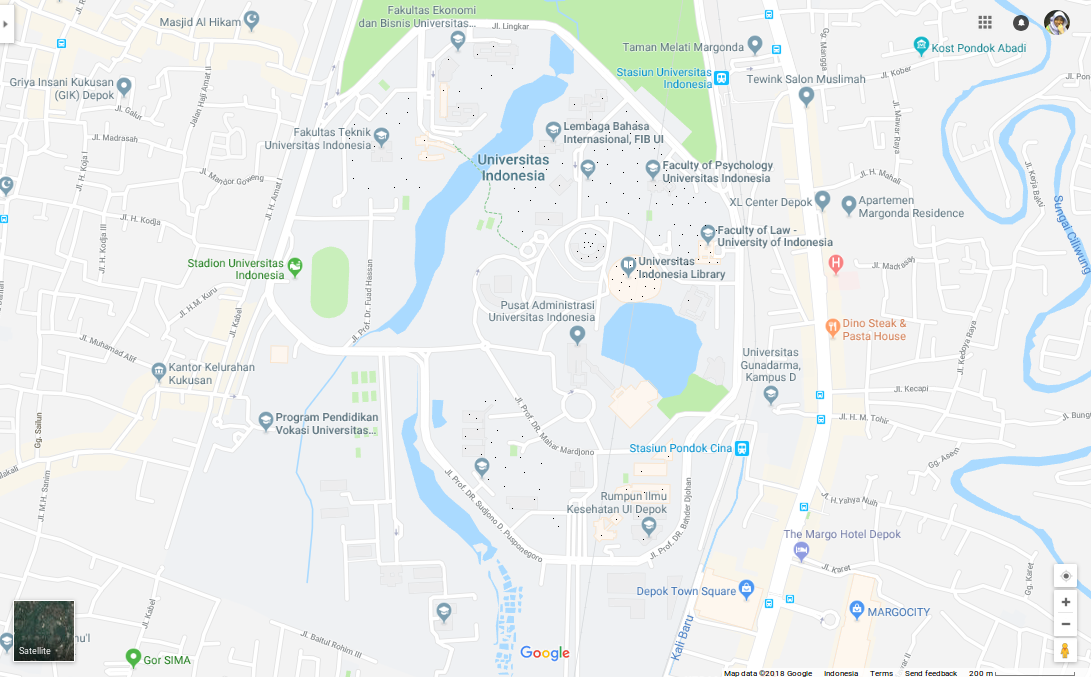
\includegraphics[width=14cm]{pics/ui-current.png}
	\caption{Peta Kampus Universitas Indonesia dengan Lokasi dari \textit{Hotspot} Saat Ini}
	\label{fig:uiCurrent}
\end{figure} 

Dalam \textit{Weighted Voronoi Diagram}, titik tersebut merupakan titik pusat dari diagram Voronoi. 

Setiap titik memiliki bobot masing-masing, yang mana bobot ini bergantung dari bandwidth dan kekuatan sinyal untuk masing-masing \textit{access point}. Bobot ini juga dihitung berdasarkan data \textit{access point} dari DSTI. 

Data \textit{access point} dari DSTI hanya menampilkan lokasi dari \textit{access point} beserta jenis \textit{router} yang digunakan, tanpa data mengenai \textit{bandwidth} dari setiap \textit{access point} tersebut. Sehingga untuk penelitian ini bobot yang digunakan hanya berdasarkan kekuatan sinyal dari setiap \textit{router}, dan \textit{bandwidth} untuk setiap \textit{router} dianggap sama.

\section{Menggambarkan Jangkauan \textit{Hotspot} pada Peta}

Dari setiap \textit{access point} digambarkan jangkauan dari \textit{access point} tersebut berupa lingkaran warna kuning. Panjang jari-jari dari lingkaran tersebut tergantung bobot dari titik pusatnya.

\begin{figure}
	\centering
	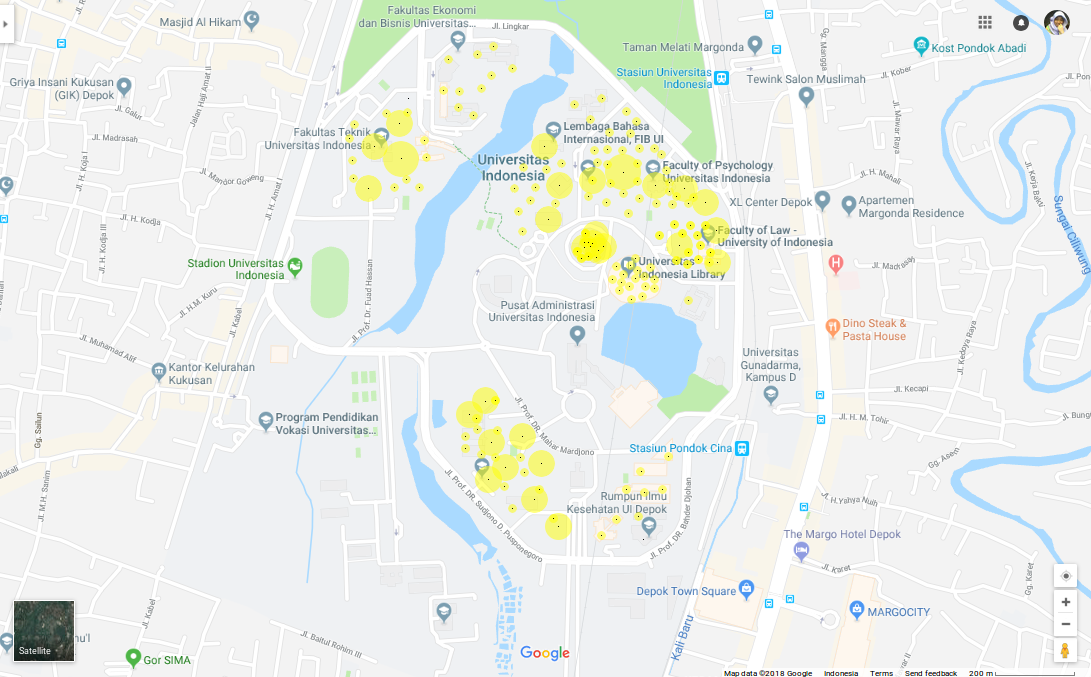
\includegraphics[width=14cm]{pics/ui-coverage.png}
	\caption{Peta Kampus Universitas Indonesia dengan Lokasi dari \textit{Hotspot} Saat Ini Beserta Jangkauannya}
	\label{fig:uiCoverage}
\end{figure} 

Untuk lingkaran yang \textit{overlapping} hal ini berarti daerah tersebut mendapatkan jangkauan dari lebih dari satu \textit{router}.

Jika peta jangkauan dari \textit{hotspot} kita terapkan pada peta \textit{demand} dari \textit{hotspot}, maka hasilnya sebagai berikut.

\begin{figure}
	\centering
	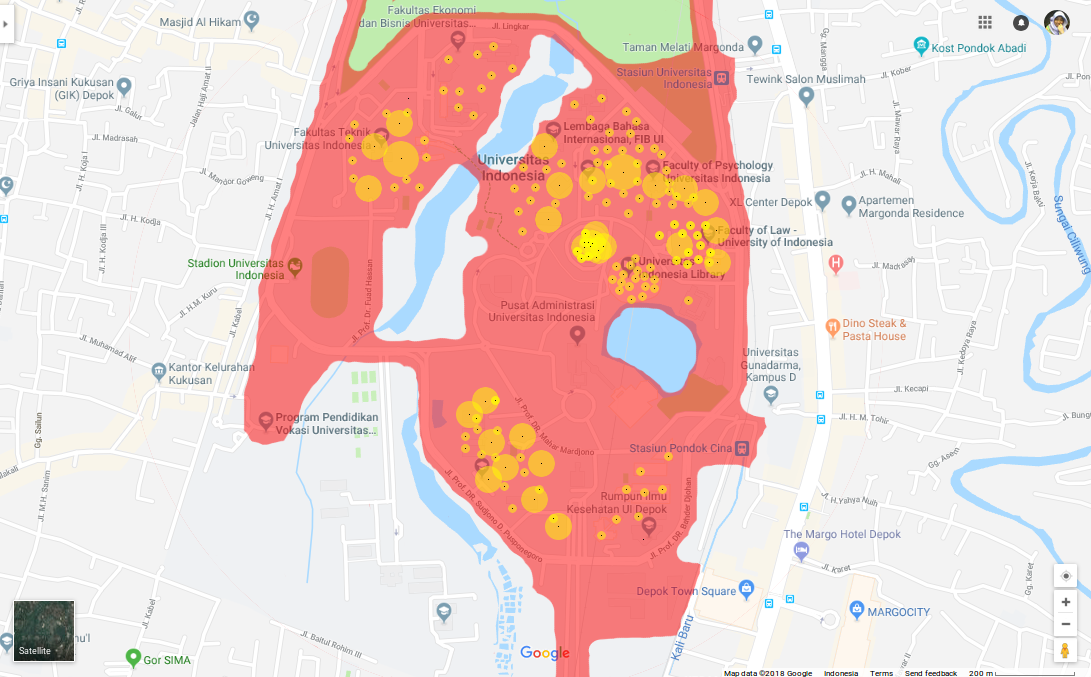
\includegraphics[width=14cm]{pics/ui-demand-coverage.png}
	\caption{Peta Kampus Universitas Indonesia dengan Lokasi dari \textit{Hotspot} Saat Ini Beserta Jangkauannya dan \textit{Demand} dari \textit{Hotspot}}
	\label{fig:uiCoverageDemand}
\end{figure} 

Dari gambar tersebut dapat kita lihat bahwa kondisi \textit{hotspot} saat ini masih belum memenuhi kebutuhan \textit{hotspot}.

\section{Menggambarkan Weighted Voronoi Diagram pada Peta}

Untuk melakukan penggambaran \textit{Weighted Voronoi Diagram} digunakan R Studio. Namun terdapat keterbatasan untuk penggambarannya yaitu gambar yang dihasilkan hanya berukuran 480x480 piksel. Dengan keterbatasan ini kemudian peta kampus {\ui} Depok dibagi menjadi beberapa bagian yang masing-masing bagiannya berukuran 480x480 piksel.

Untuk setiap bagian dalam peta, setiap lokasi dari \textit{access point} digambarkan ke dalam R studio berdasarkan lokasi koordinatnya. Setiap koordinat dari titik tersebut dituliskan dalam sebuah file yang kemudian akan dibaca oleh progam (sesuatu siapa namanya lupa).

Bobot untuk setiap titik tersebut juga disimpan dalam sebuah file berbeda. Nilai dari bobot tidak harus bilangan bulat, akan tetapi bisa berupa bilangan pecahan. 

Program tersebut kemudian melakukan \textit{plotting} dari data lokasi serta bobot dari setiap titik ke dalam gambar berukuran 480x480 piksel.

Setelah itu program ini akan menggambarkan \textit{Weighted Voronoi Diagram} dari kumpulan titik tersebut menjadi gambar ber-\textit{format} .jpeg.

Gambar \textit{Weighted Voronoi Diagram} yang dihasilkan dari program tersebut kemudian diubah menjadi gambar ber-\textit{format} .png menggunakan suatu aplikasi \textit{image converter} (link online). Gambar tersebut kemudian di \textit{overlay} pada gambar peta {\ui}.

Hal tersebut dilakukan untuk setiap potongan gambar dari peta {\ui} sehingga \textit{Weighted Voronoi Diagram} dari seluruh lokasi \textit{access point} tergambarkan dalam peta.

\section{Evaluasi Coverage \textit{Hotspot} Terhadap Demand}
Peta {\ui} yang sudah terdapat \textit{Weighted Voronoi Diagram} di dalamnya kemudian dievaluasi secara visual untuk mengetahui daerah mana yang belum mendapatkan jangkauan \textit{hotspot}.

Evaluasi yang dilakukan adalah dengan melihat apakah setiap daerah yang berwarna merah ada di dalam lingkaran berwarna kuning. Jika semua daerah yang berwarna merah sudah berada di dalam lingkaran berwarna kuning, maka setiap \textit{demand area} sudah mendapatkan jaringan hotspot. Namun jika ada daerah berwarna merah yang tidak berada dalam lingkaran berwarna kuning, maka perlu ditambahkan \textit{access point} baru di daerah tersebut.

\section{Menambahkan Lokasi \textit{Hotspot} Baru pada Daerah yang Belum Ter-cover Beserta Bobotnya}

Untuk daerah berwarna merah yang tidak berada pada lingkaran berwarna kuning, maka perlu ditambahkan titik baru atau \textit{access point} baru di dalamnya. Untuk menentukan di mana lokasi dari titik baru tersebut maka dilakukan analisis terhadap diagram Voronoi pada daerah tersebut. Lokasi baru dari \textit{access point} berada pada ujung diagram Voronoi, yang mana ujung diagram Voronoi adalah lokasi terjauh dari setiap titik-titik di sekitarnya. 

Hal tersebut dilakukan untuk setiap daerah berwarna merah yang tidak berada dalam lingkaran berwarna kuning. 

Setiap titik diberikan bobot yang sama dengan bobot terkecil diantara titik-titik yang ada. Hal ini ditujukan untuk mengambil seminimal mungkin \textit{cost} yang harus dikeluarkan untuk menambahkan \textit{access point} baru. 

\section{Menggambarkan Jangkauan untuk \textit{Hotspot} Baru pada Peta}

Untuk setiap titik baru yang ditambahkan dalam peta, kemudian digambarkan lingkaran kuning di sekitarnya yang menggambarkan jangkauan dari \textit{access point} tersebut seperti yang dilakukan dalam langkah sebelumnya.

\section{Menggambarkan Weighted Voronoi Diagram Baru}

Proses untuk menggambarkan \textit{Weighted Voronoi Diagram} sama dengan pada tahap sebelumnya. Dalam proses ini maka akan terbentuk diagram-diagram Voronoi baru, dan bentuk dari diagram-diagram Voronoi sebelumnya akan berubah. Hal ini dikarenakan...

\section{Evaluasi Coverage \textit{Hotspot} Baru Terhadap Demand}

Hasil dari pemetaan diagram Voronoi pada peta kemudian di-evaluasi kembali untuk mencari daerah mana yang belum mendapatkan jangkauan hotspot. Kemudian dilakukan hal yang sama sampai setiap daerah berwarna merah berada di dalam lingkaran-lingkaran berwarna kuning.

\section{Generate Weighted Voronoi Diagram}

Program tersebut menggambar suatu persegi yang berisi sepuluh titik berbobot yang lokasi dan bobotnya diambil secara random. Dari sepuluh titik berbobot itu kemudian digambarkan weighted voronoi diagramnya. \cite{voronoi.R}

